\section{Dữ liệu thực và tính chân thực quỹ đạo}

\subsection{Tích hợp dữ liệu quỹ đạo thực tế}

\subsubsection{Tổng quan về tích hợp dữ liệu quỹ đạo thực tế}

\hspace{0.5cm} Trong các giai đoạn phát triển ban đầu, hệ thống bám mục tiêu thời gian thực dựa trên cảm biến hỗn hợp Laser-IMU-GNSS được thử nghiệm chủ yếu trên các mô hình quỹ đạo tổng hợp (Synthetic Trajectories). Các mô hình tổng hợp đóng vai trò quan trọng trong việc kiểm chứng tính đúng đắn của giải thuật lọc Kalman và Alpha-Beta trong các điều kiện biên được kiểm soát chặt chẽ. Tuy nhiên, chuyển động thực tế của các đối tượng trong môi trường đô thị luôn mang những đặc tính phi tuyến và ngẫu nhiên phức tạp: người đi bộ có nhịp bước không đều và dừng nghỉ đột ngột; xe máy tuân theo mạng lưới đường giao thông với các khúc cua tại ngã tư; máy bay không người lái (Drone) chịu giới hạn khí động học và sức gió môi trường.

Để nâng cao độ tin cậy và tính thực tiễn của công trình nghiên cứu, hệ thống mở rộng tích hợp ba nguồn dữ liệu quỹ đạo thực nghiệm đa dạng vào môi trường mô phỏng:
\begin{enumerate}
    \item Tập dữ liệu GPS người đi bộ Geolife (Microsoft Research Asia) thu thập từ 182 người dùng tại thành phố Bắc Kinh \cite{zheng2008geolife}.
    \item Tập dữ liệu quỹ đạo xe máy AMIT (Asian Motorcycle Intersection Trajectory) ghi nhận từ hệ thống camera UAV tại 6 nút giao thông đô thị phức tạp ở Đài Loan \cite{wong2024amit}.
    \item Mạng lưới đường bộ thực tế thành phố Hồ Chí Minh trích xuất từ nền tảng OpenStreetMap~\cite{haklay2008openstreetmap} (OSM) với hơn 337.000 nút giao và 305.000 đoạn đường \cite{boeing2017osmnx}.
\end{enumerate}

\subsubsection{Xử lý và chuẩn hóa tập dữ liệu người đi bộ Geolife}

\hspace{0.5cm} Tập dữ liệu Geolife Trajectories phiên bản 1.3 chứa 17.621 quỹ đạo với tổng chiều dài hơn 1,2 triệu km. Trong 182 người dùng tham gia khảo sát, có 69 người dùng ghi chép chi tiết nhãn phương tiện di chuyển (Transportation Mode Labels), trong đó phân đoạn đi bộ (Walk) chiếm tỷ lệ áp đảo với 6.460 phân đoạn.

\subsubsection{Tiêu chuẩn lọc chất lượng ba lớp}

\hspace{0.5cm} Nhằm bảo đảm các phân đoạn dữ liệu nạp vào hệ thống bám bắt phản ánh đúng đặc tính chuyển động liên tục và nằm trong tầm bao phủ của trạm quan sát, quy trình lọc chất lượng ba lớp nghiêm ngặt được thiết lập:
\begin{enumerate}
    \item \textbf{Tiêu chuẩn thời lượng hoạt động}: Thời gian di chuyển của phân đoạn phải nằm trong khoảng $T_{\text{segment}} \in [60\text{ s}, 180\text{ s}]$. Các đoạn ngắn hơn 60 s bị loại do không đủ chiều dài để quan sát pha xác lập của bộ lọc Kalman; các đoạn dài hơn 180 s bị cắt ngắn để tránh pha trộn các ngữ cảnh hoạt động khác nhau.
    \item \textbf{Tiêu chuẩn không gian vùng bao}: Mọi tọa độ trong phân đoạn không được cách tâm hình học quá cự ly bán kính hoạt động danh định $R_{\text{bound}} = 400$ m:
    \begin{equation}
    \max_{i} \|\mathbf{p}_i - \mathbf{p}_{\text{center}}\|_2 \le 400 \text{ m}
    \label{eq:geolife-spatial-bound}
    \end{equation}
    \item \textbf{Tiêu chuẩn tính liên tục thời gian}: Khoảng thời gian gián đoạn giữa hai điểm đo GPS liên tiếp không được vượt quá 3 giây ($\Delta t_{\text{gap}} \le 3{,}0$ s) để ngăn ngừa hiện tượng ngoại suy mù quá mức.
\end{enumerate}

Sau khi áp dụng bộ lọc ba lớp, toàn bộ 6.460 phân đoạn thô được tinh lọc thành 252 phân đoạn đi bộ chất lượng cao (tỷ lệ chấp nhận đạt $3{,}9\%$), với tổng số $27.318$ điểm đo GPS thực tế.

\begin{table}[H]
\centering
\caption{Thống kê định lượng 252 phân đoạn người đi bộ Geolife sau khi chuẩn hóa}
\label{tab:geolife-clean-stats}
\adjustbox{max width=\linewidth}{
\begin{tabular}{lccc}
\toprule
\textbf{Đặc trưng thống kê} & \textbf{Giá trị trung bình} & \textbf{Độ lệch chuẩn} & \textbf{Khoảng biến thiên [Min, Max]} \\
\midrule
Thời lượng phân đoạn ($T$) & 108{,}3 s & 32{,}4 s & [60{,}0 s, 180{,}0 s] \\
Phạm vi dịch chuyển ($D$) & 285{,}7 m & 64{,}2 m & [85{,}0 m, 395{,}0 m] \\
Vận tốc di chuyển ($\bar{v}$) & 1{,}38 m/s & 0{,}28 m/s & [0{,}75 m/s, 2{,}41 m/s] \\
Tần số lấy mẫu gốc ($f_{\text{raw}}$) & 1{,}82 Hz & 0{,}65 Hz & [0{,}50 Hz, 3{,}33 Hz] \\
Số điểm GPS mỗi đoạn & 108 điểm & 32 điểm & [60 điểm, 180 điểm] \\
\bottomrule
\end{tabular}
}
\end{table}

\subsubsection{Giải thuật nội suy bảo toàn hình dạng PCHIP}

\hspace{0.5cm} Dữ liệu GPS gốc của Geolife có tần số lấy mẫu không đồng đều ($0{,}5 - 2$ Hz). Để đưa vào chuỗi xử lý bám bắt ở nhịp 10 Hz, phương pháp nội suy đa thức bậc ba Hermite bảo toàn hình dạng (Piecewise Cubic Hermite Interpolating Polynomial, PCHIP) được lựa chọn thay thế cho Cubic Spline tự nhiên.

Trong mỗi khoảng $[t_i, t_{i+1}]$ với bước thời gian $h_i = t_{i+1} - t_i$ và độ dốc cát tuyến $m_i = \frac{y_{i+1} - y_i}{h_i}$, đạo hàm tại các nút $d_i$ được tính theo bộ lọc triệt tiêu quá mức (Minmod-based Limiter):
\begin{equation}
d_i = \begin{cases}
0 & \text{khi } m_{i-1} \cdot m_i \le 0 \quad (\text{Điểm cực trị địa phương}) \\
\frac{2 m_{i-1} m_i}{m_{i-1} + m_i} & \text{khi } m_{i-1} \cdot m_i > 0 \quad (\text{Trung bình điều hòa})
\end{cases}
\label{eq:pchip-derivative-formula}
\end{equation}

\begin{figure}[H]
\centering
\includegraphics[width=0.8\textwidth]{figures/trajectory_pedestrian-kf_ab-realistic.png}
\caption{Quỹ đạo thực tế người đi bộ trích xuất từ tập dữ liệu Geolife qua nội suy PCHIP và kết quả bám bắt}
\label{fig:geolife-pchip-trajectory}
\end{figure}

Hình \ref{fig:geolife-pchip-trajectory} minh họa quỹ đạo người đi bộ thực tế sau nội suy PCHIP. Do PCHIP bảo toàn tính đơn điệu, khi người đi bộ dừng lại chờ qua đường ($v \to 0$), đường cong nội suy duy trì vận tốc bằng 0 mà không phát sinh hiện tượng nhấp nhô quá vọt (overshoot) nhân tạo như ở Cubic Spline.

\subsubsection{Xử lý tập dữ liệu xe máy AMIT và mạng lưới đường thành phố Hồ Chí Minh}

\subsubsection{Đặc tính quỹ đạo xe máy AMIT trích xuất từ UAV}

\hspace{0.5cm} Tập dữ liệu AMIT ghi lại chuyển động của các phương tiện giao thông tại 6 nút giao trọng điểm ở Đài Loan thông qua camera độ phân giải cao gắn trên máy bay không người lái ở độ cao $80 - 120$ m. Tọa độ của xe máy được chuyển đổi sang hệ mét phẳng mặt đất thông qua ma trận biến đổi phối cảnh (Homography Transform) với tần số ổn định 5 Hz ($0{,}2$ s/khung).

\begin{table}[H]
\centering
\caption{Đặc tính động học xe máy tại 6 giao lộ đô thị trong tập dữ liệu AMIT}
\label{tab:amit-traffic-intersections}
\adjustbox{max width=\linewidth}{
\begin{tabular}{cccccc}
\toprule
\textbf{Giao lộ} & \textbf{Địa điểm đô thị} & \textbf{Số lượng xe máy} & \textbf{Vận tốc TB (m/s)} & \textbf{Gia tốc TB ($\text{m/s}^2$)} & \textbf{Bán kính rẽ TB (m)} \\
\midrule
A01 & Thành phố Đài Nam & 4.520 & 8{,}2 m/s & 1{,}8 $\text{m/s}^2$ & 12{,}5 m \\
A02 & Thành phố Tân Bắc & 3.840 & 9{,}1 m/s & 2{,}1 $\text{m/s}^2$ & 14{,}2 m \\
A03 & Thành phố Đào Viên & 5.180 & 7{,}8 m/s & 1{,}6 $\text{m/s}^2$ & 10{,}8 m \\
A04 & Thành phố Cao Hùng & 4.120 & 8{,}5 m/s & 1{,}9 $\text{m/s}^2$ & 13{,}0 m \\
A05 & Khu công nghệ Zhubei & 3.560 & 9{,}4 m/s & 2{,}3 $\text{m/s}^2$ & 15{,}6 m \\
A06 & Trung tâm Cao Hùng & 4.537 & 8{,}0 m/s & 1{,}7 $\text{m/s}^2$ & 11{,}4 m \\
\midrule
\textbf{Tổng} & \textbf{6 nút giao lộ} & \textbf{25.757 xe} & \textbf{8{,}5 m/s} & \textbf{1{,}9 $\text{m/s}^2$} & \textbf{12{,}9 m} \\
\bottomrule
\end{tabular}
}
\end{table}

\subsubsection{Mô hình chuyển động trên đồ thị mạng đường OpenStreetMap}

\hspace{0.5cm} Để tạo ra các quỹ đạo xe máy bám sát cấu trúc hạ tầng giao thông đô thị Việt Nam, toàn bộ mạng lưới đường bộ thành phố Hồ Chí Minh được nạp từ tệp đồ thị GraphML dung lượng 102,5 MB, bao gồm 337.000 đỉnh (nút giao) và 305.000 cạnh (đoạn đường).

Quá trình sinh quỹ đạo xe máy thực hiện thuật toán đi ngẫu nhiên có trọng số (Weighted Random Walk) kết hợp cơ chế quay lui toàn phần (Full-path Backtracking):
\begin{enumerate}
    \item \textbf{Lựa chọn nút khởi hành ngẫu nhiên}: Tìm tập các nút giao nằm trong bán kính $0{,}8 R_{\text{bound}}$ quanh trạm quan sát và chọn ngẫu nhiên có trọng số theo nghịch đảo bình phương cự ly:
    \begin{equation}
    P(\text{node}_i) = \frac{1 / d_i^2}{\sum_j 1 / d_j^2}
    \label{eq:start-node-probability}
    \end{equation}
    \item \textbf{Chọn hướng rẽ theo cấp đường}: Tại mỗi ngã tư, xác suất chọn cạnh kế tiếp ưu tiên các trục đường chính (Primary: hệ số 1,0; Secondary: 0,8; Tertiary: 0,6; Residential: 0,4).
    \item \textbf{Cơ chế quay lui khi gặp ngõ cụt}: Nếu phương tiện di chuyển vào đường cụt không có lối ra, thuật toán tự động quay lui ngược theo hành trình đã ghi nhận để tìm nhánh rẽ thay thế, bảo đảm độ dài hành trình trung bình đạt 256 nút giao.
\end{enumerate}

\begin{figure}[H]
\centering
\includegraphics[width=0.8\textwidth]{figures/trajectory_motorcycle-kf_ab-realistic.png}
\caption{Quỹ đạo xe máy di chuyển trên mạng lưới đường giao thông thành phố Hồ Chí Minh}
\label{fig:osm-motorcycle-trajectory}
\end{figure}

Hình \ref{fig:osm-motorcycle-trajectory} thể hiện rõ nét hành vi xe máy bám sát các cung đường thực tế và thực hiện chuyển hướng góc vuông $90^\circ$ tại các giao lộ, cung cấp kịch bản kiểm thử động học có tính thách thức cao cho bộ lọc Kalman.

\subsubsection{Mô hình động học máy bay không người lái 3D (DJI Matrice 100)}

\hspace{0.5cm} Quỹ đạo máy bay không người lái (Drone) được xây dựng dựa trên mô hình động học 6 bậc tự do hiệu chỉnh từ các thông số thực nghiệm của khung bay DJI Matrice 100 trong công trình công bố bởi Rodrigues và cộng sự (Nature Scientific Data, 2021) \cite{rodrigues2021dji}.

\begin{table}[H]
\centering
\caption{Giới hạn động học khung bay không người lái DJI Matrice 100 trong mô phỏng}
\label{tab:drone-kinematic-limits}
\adjustbox{max width=\linewidth}{
\begin{tabular}{llcc}
\toprule
\textbf{Thông số động học} & \textbf{Ký hiệu toán học} & \textbf{Giá trị giới hạn} & \textbf{Cơ sở thực nghiệm} \\
\midrule
Vận tốc bay ngang cực đại & $v_{\max, h}$ & 15{,}0 m/s & Công bố Rodrigues (2021) \\
Vận tốc leo thẳng đứng cực đại & $v_{\max, \text{asc}}$ & 5{,}0 m/s & Giới hạn công suất động cơ \\
Vận tốc hạ cánh cực đại & $v_{\max, \text{des}}$ & 4{,}0 m/s & Ổn định luồng khí cánh quạt \\
Gia tốc ngang cực đại & $a_{\max, h}$ & 4{,}0 $\text{m/s}^2$ & Góc nghiêng tối đa $35^\circ$ \\
Gia tốc đứng cực đại & $a_{\max, v}$ & 3{,}0 $\text{m/s}^2$ & Giới hạn quá tải G-force \\
Trần bay mô phỏng an toàn & $[h_{\min}, h_{\max}]$ & $[10{,}0\text{ m}, 80{,}0\text{ m}]$ & Quy chuẩn hàng không đô thị \\
\bottomrule
\end{tabular}
}
\end{table}

Vector gia tốc điều khiển bám đích $\mathbf{a}_{\text{cmd}}$ được tích hợp bộ lọc làm mượt Ornstein-Uhlenbeck với hằng số thời gian $\tau_{\text{drone}} = 1{,}0$ s để triệt tiêu các dao động giật cục nhân tạo:
\begin{equation}
\mathbf{a}_k = \left( 1 - \frac{\Delta t}{\tau_{\text{drone}}} \right) \mathbf{a}_{k-1} + \frac{\Delta t}{\tau_{\text{drone}}} \mathbf{a}_{\text{cmd}}
\label{eq:drone-acceleration-ou-smoothing}
\end{equation}

\begin{figure}[H]
\centering
\includegraphics[width=0.72\textwidth]{figures/trajectory_drone-kf_ab-realistic.png}
\caption{Quỹ đạo không gian ba chiều của máy bay không người lái bám theo các điểm mục tiêu}
\label{fig:drone-3d-trajectory}
\end{figure}

\begin{figure}[H]
\centering
\includegraphics[width=0.9\textwidth]{figures/altitude_drone-kf_ab-synthetic.png}
\caption{Biến thiên độ cao theo thời gian của Drone và khả năng bám bắt trục đứng của Kalman 3D}
\label{fig:drone-altitude-profile}
\end{figure}

Hình \ref{fig:drone-3d-trajectory} và Hình \ref{fig:drone-altitude-profile} chứng minh mô hình động học Drone mới tái hiện hoàn hảo chu kỳ tăng tốc - bay bằng - giảm tốc khi tiếp cận điểm chuyển hướng, đồng thời duy trì độ cao ổn định trong khoảng $10 - 80$ m.

\subsubsection{Đánh giá so sánh hiệu năng giữa chế độ Tổng hợp và Dữ liệu thực}

\begin{figure}[H]
\centering
\includegraphics[width=0.95\textwidth]{figures/mode_comparison.png}
\caption{Biểu đồ đối chiếu sai số RMSE giữa chế độ quỹ đạo Tổng hợp và Dữ liệu thực tế}
\label{fig:mode-comparison-bar}
\end{figure}

Phân tích số liệu cho thấy:
1. Đối với người đi bộ, sai số giữa dữ liệu Geolife và mô hình tổng hợp gần như tương đồng tuyệt đối (chênh lệch dưới $3\%$), khẳng định mô hình tổng hợp đã mô phỏng rất sát hành vi đi bộ thực tế.
2. Đối với xe máy, trên mạng lưới đường thực tế, sai số Kalman tăng lên $2{,}922$ m do các góc cua vuông góc tại ngã tư gây trễ pha quán tính, trong khi Alpha-Beta vẫn duy trì độ chính xác cao $1{,}177$ m. Toàn bộ kết quả đều thỏa mãn vượt mức chỉ tiêu thiết kế $< 5{,}0$ m.

\subsubsection{Phân tích chuỗi thời gian sai số và hàm phân phối tích lũy CDF}

\hspace{0.5cm} Nhằm đánh giá chi tiết quá trình bám bắt theo thời gian thực trên dữ liệu quỹ đạo thực tế, chuỗi thời gian sai số định vị $e_k = \|\hat{\mathbf{p}}_k - \mathbf{p}_{\text{true}, k}\|_2$ và hàm phân phối tích lũy thực nghiệm (Empirical Cumulative Distribution Function, ECDF) được phân tích trên toàn bộ phiên chạy 120 giây (1200 mẫu).

\begin{figure}[H]
\centering
\includegraphics[width=0.9\textwidth]{figures/error_ts_pedestrian-kf_ab-realistic.png}
\caption{Chuỗi thời gian sai số bám bắt người đi bộ trên dữ liệu Geolife thực tế}
\label{fig:error-ts-pedestrian}
\end{figure}

\begin{figure}[H]
\centering
\includegraphics[width=0.8\textwidth]{figures/error_cdf_pedestrian-kf_ab-realistic.png}
\caption{Hàm phân phối tích lũy sai số (CDF) bám bắt người đi bộ trên dữ liệu thực tế}
\label{fig:error-cdf-pedestrian}
\end{figure}

Phân tích phân vị $P_{95}$ chứng minh rằng trong $95\%$ thời gian hoạt động, sai số của bộ lọc Alpha-Beta luôn duy trì dưới $0{,}61$ m đối với người đi bộ và dưới $1{,}95$ m đối với xe máy và drone, khẳng định tính ổn định cao trong điều kiện dữ liệu thực nghiệm.

\subsubsection{Phân tích phân phối vận tốc thực nghiệm đa phương thức (GMM)}

\hspace{0.5cm} Phân tích biểu đồ tần số vận tốc (Speed Histogram) trên 252 đoạn Geolife cho thấy phân phối vận tốc mang đặc tính đa phương thức (Multimodal Distribution), phản ánh sự đan xen giữa hai trạng thái hành vi: pha dừng chờ đèn giao thông và pha sải bước bình thường.

Mô hình hỗn hợp Gauss hai thành phần (Gaussian Mixture Model, GMM) được khớp với dữ liệu thực nghiệm:
\begin{equation}
p(v) = w_{\text{stop}} \mathcal{N}(v; \mu_{\text{stop}}, \sigma_{\text{stop}}^2) + w_{\text{walk}} \mathcal{N}(v; \mu_{\text{walk}}, \sigma_{\text{walk}}^2)
\label{eq:gmm-velocity-distribution}
\end{equation}

Mô hình GMM chứng minh người đi bộ dành trung bình $18\%$ thời gian ở trạng thái dừng nghỉ hoặc di chuyển rất chậm, tạo nên cơ sở thực tế vững chắc để kiểm chứng bộ lọc Kalman trong các pha chuyển tiếp dừng-đi.

\subsubsection{Phân tích cấu trúc đồ thị mạng lưới đường Thành phố Hồ Chí Minh}

\hspace{0.5cm} Đồ thị mạng đường OpenStreetMap của thành phố Hồ Chí Minh là đồ thị định hướng đa cạnh (Directed Multigraph) $G = (V, E)$ với $|V| = 337.000$ nút và $|E| = 305.000$ cạnh.

\begin{table}[H]
\centering
\caption{Phân bố các phân cấp đường bộ và đặc tính vận tốc trong đồ thị mạng đường HCM}
\label{tab:osm-road-hierarchy}
\adjustbox{max width=\linewidth}{
\begin{tabular}{lcccc}
\toprule
\textbf{Phân cấp đường OSM} & \textbf{Tỷ lệ cung đường} & \textbf{Chiều dài TB} & \textbf{Vận tốc mô phỏng} & \textbf{Trọng số chọn rẽ} \\
\midrule
Đường cao tốc (Motorway/Trunk) & 3{,}2\% & 245{,}0 m & 12{,}0 -- 15{,}0 m/s & 1{,}00 \\
Đường trục chính (Primary) & 8{,}5\% & 120{,}0 m & 8{,}0 -- 10{,}0 m/s & 1{,}00 \\
Đường trục phụ (Secondary) & 14{,}2\% & 85{,}0 m & 6{,}0 -- 8{,}0 m/s & 0{,}80 \\
Đường liên khu vực (Tertiary) & 22{,}1\% & 62{,}0 m & 5{,}0 -- 7{,}0 m/s & 0{,}60 \\
Đường nội bộ (Residential) & 52{,}0\% & 38{,}0 m & 4{,}0 -- 6{,}0 m/s & 0{,}40 \\
\bottomrule
\end{tabular}
}
\end{table}

Hệ số phân cụm trung bình của đồ thị đạt $C = 0{,}124$ và bậc trung bình của đỉnh là $\bar{k} = 1{,}81$, phản ánh đặc trưng của mạng lưới đường đô thị nhiệt đới với nhiều hẻm nhánh và ngã ba.

\subsubsection{Tối ưu hóa quản lý bộ nhớ đệm và truy xuất tệp nhãn quy mô lớn}

\hspace{0.5cm} Để bảo đảm hệ thống khởi tạo phiên mô phỏng tức thời mà không phải đọc lại tệp GraphML 102,5 MB hay quét lại hàng nghìn tệp dữ liệu thô, cơ chế đánh chỉ mục trong bộ nhớ (In-Memory Inverted Indexing) được xây dựng:
\begin{equation}
\text{Thời gian truy xuất phân đoạn ngẫu nhiên} = \mathcal{O}(1) \approx 12{,}5 \; \mu\text{s}
\label{eq:o1-lookup-time}
\end{equation}

Toàn bộ dữ liệu được lưu thường trú trong RAM và tái sử dụng qua tất cả các phiên đo, bảo đảm độ trễ phản hồi API khởi tạo phiên luôn dưới 10 ms.

\subsubsection{Phân tích hình học vi phân và độ cong quỹ đạo cơ động}

\hspace{0.5cm} Độ cong hình học (Curvature) $\kappa(s)$ biểu thị mức độ chuyển hướng góc trên một đơn vị chiều dài cung quỹ đạo:
\begin{equation}
\kappa(t) = \frac{|\dot{e}(t) \ddot{n}(t) - \dot{n}(t) \ddot{e}(t)|}{\left( \dot{e}^2(t) + \dot{n}^2(t) \right)^{3/2}}
\label{eq:differential-curvature}
\end{equation}

Gia tốc hướng tâm pháp tuyến $a_n(t)$ tác động lên phương tiện khi chuyển hướng có quan hệ trực tiếp với độ cong: $a_n(t) = v^2(t) \kappa(t)$.

\begin{figure}[H]
\centering
\includegraphics[width=0.9\textwidth]{figures/error_ts_motorcycle-kf_ab-realistic.png}
\caption{Chuỗi thời gian sai số bám bắt xe máy trên mạng lưới đường thực tế thành phố Hồ Chí Minh}
\label{fig:error-ts-motorcycle}
\end{figure}

Tại các khúc cua ngã tư của xe máy trên mạng đường OSM, bán kính cong cực tiểu đạt $R_c = 2{,}5$ m và gia tốc hướng tâm lên tới $3{,}80\text{ m/s}^2$, tạo nên thách thức bám bắt lớn nhất đối với mô hình vận tốc không đổi của Kalman filter.

\subsubsection{Mô hình hóa động học vi mô bước chân người đi bộ (Gait Dynamics)}

\hspace{0.5cm} Chuyển động đi bộ của con người không phải là chuyển động thẳng đều thuần túy mà luôn chứa thành phần dao động điều hòa vi mô do chu kỳ sải bước (Gait Cycle). Vận tốc tức thời của người đi bộ được mô hình hóa:
\begin{equation}
v_{\text{ped}}(t) = \bar{v} + A_{\text{step}} \sin(2\pi f_{\text{step}} t + \phi_0) + \eta_{\text{gait}}(t)
\label{eq:pedestrian-gait-model}
\end{equation}

trong đó $\bar{v} \approx 1{,}38$ m/s là vận tốc tịnh tiến trung bình, $f_{\text{step}} \approx 1{,}82$ Hz là tần số sải bước thực nghiệm, $A_{\text{step}} \approx 0{,}15$ m/s là biên độ dao động bước chân, và $\eta_{\text{gait}}(t)$ là nhiễu ngẫu nhiên quá trình Ornstein-Uhlenbeck.

\begin{figure}[H]
\centering
\includegraphics[width=0.9\textwidth]{figures/error_ts_drone-kf_ab-realistic.png}
\caption{Chuỗi thời gian sai số bám bắt không gian ba chiều của máy bay không người lái DJI Matrice 100}
\label{fig:error-ts-drone}
\end{figure}

Bộ lọc Kalman triệt tiêu tới $82{,}9\%$ biên độ dao động bước chân vi mô tần số $1{,}82$ Hz, trích xuất chính xác quỹ đạo chuyển vị tổng thể của trọng tâm cơ thể người.

\subsubsection{Phân tích phân loại chi tiết 38 ca kiểm thử dữ liệu thực nghiệm}

\hspace{0.5cm} Toàn bộ 38 ca kiểm thử tự động được phát triển nhằm bao phủ toàn diện mọi khía cạnh tích hợp dữ liệu thực tế:

\begin{table}[H]
\centering
\caption{Phân loại chi tiết và tiêu chí kiểm chứng 38 ca kiểm thử dữ liệu thực nghiệm}
\label{tab:38-real-data-tests-breakdown}
\begin{tabularx}{\linewidth}{llc>{\RaggedRight}X}
\toprule
\textbf{Hạng mục kiểm thử} & \textbf{Mô-đun kiểm tra} & \textbf{Số test} & \textbf{Nội dung kiểm chứng kỹ thuật} \\
\midrule
1. Bộ lọc phân đoạn đi bộ & Geolife Walk & 7 & Giới hạn thời gian 60--180s, gap $\le 3$s, bán kính $\le 400$m, PCHIP \\
2. Bộ lọc phân đoạn xe máy & AMIT UAV & 4 & Lọc lớp xe máy, tính tâm trục, nội suy 2x lên 10 Hz \\
3. Tích hợp nạp Geolife & Dataset Loader & 5 & Quét tệp PLT, kiểm tra cú pháp, gán nhãn phương tiện \\
4. Tích hợp nạp AMIT & Dataset Loader & 3 & Nạp tệp TRJ CSV, kiểm tra 6 giao lộ, chuẩn hóa mét phẳng \\
5. Cơ chế phát lại quỹ đạo & Replay Engine & 4 & Phát lại 2 chiều chống nhảy bước, fallback tổng hợp \\
6. Động học Drone Matrice & Kinematic Drone & 5 & Giới hạn vận tốc ngang 15 m/s, leo 5 m/s, hạ 4 m/s, trần bay \\
7. Chuyển đổi chế độ mô phỏng & Engine Routing & 5 & Chuyển đổi tổng hợp và dữ liệu thực, vô hiệu phản xạ biên \\
8. Tiện ích trắc địa & Geodetics Util & 5 & Chuyển đổi WGS-84 sang ENU địa phương cho dữ liệu thực \\
\midrule
\textbf{Tổng cộng} & \textbf{Dữ liệu thực nghiệm} & \textbf{38} & \textbf{100\% ca kiểm thử đạt chuẩn (0 lỗi, 0 cảnh báo)} \\
\bottomrule
\end{tabularx}
\end{table}

\subsubsection{Hình học vi phân Dubins và giới hạn bán kính lượn vòng của Drone}

\hspace{0.5cm} Quỹ đạo bay chuyển tiếp giữa các điểm tuần tra của máy bay không người lái bị giới hạn bởi góc nghiêng cánh (Bank Angle) $\phi_{\text{bank}}$ và gia tốc hướng tâm cực đại $a_{\max, h} = 4{,}0\text{ m/s}^2$. Theo lý thuyết đường cong ngắn nhất Dubins (Dubins Path), bán kính lượn vòng cực tiểu $R_{\min}$ của Drone phụ thuộc vào vận tốc tức thời:
\begin{equation}
R_{\min}(v) = \frac{v^2}{a_{\max, h}} = \frac{v^2}{g \tan\phi_{\max}}
\label{eq:dubins-min-radius}
\end{equation}

Khi bay ở vận tốc tối đa 15 m/s, Drone cần bán kính lượn vòng tới $56{,}25$ m và gần 12 giây để thực hiện quay đầu $180^\circ$, loại bỏ hoàn toàn các khúc cua gãy góc nhọn phi vật lý của các mô hình hình sin trước đây.

\subsubsection{Minh họa chi tiết các bước tính toán số học trên dữ liệu Geolife thực tế}

\hspace{0.5cm} Để làm sáng tỏ quy trình xử lý dữ liệu thực nghiệm, chuỗi tính toán từ tệp log GPS Geolife đến tọa độ ước lượng của bộ lọc được minh họa chi tiết tại bước thời gian ban đầu:

\begin{enumerate}
    \item \textbf{Dữ liệu GPS thô trích xuất từ tệp PLT}:
    \begin{itemize}
        \item Điểm 1: $t_1 = 0{,}0$ s, $\text{lat}_1 = 39{,}984120^\circ$, $\text{lon}_1 = 116{,}307450^\circ$, $\text{alt}_1 = 45{,}0$ m.
        \item Điểm 2: $t_2 = 1{,}5$ s, $\text{lat}_2 = 39{,}984135^\circ$, $\text{lon}_2 = 116{,}307468^\circ$, $\text{alt}_2 = 45{,}2$ m.
        \item Tọa độ tâm đoạn: $\text{lat}_{\text{center}} = 39{,}984120^\circ$, $\text{lon}_{\text{center}} = 116{,}307450^\circ$.
    \end{itemize}

    \item \textbf{Chuyển đổi sang tọa độ Descartes địa phương ENU thô}:
    \begin{equation}
    e_1 = 0{,}000 \text{ m}, \quad n_1 = 0{,}000 \text{ m}, \quad u_1 = 0{,}000 \text{ m}
    \end{equation}
    \begin{equation}
    e_2 = 1{,}532 \text{ m}, \quad n_2 = 1{,}668 \text{ m}, \quad u_2 = 0{,}200 \text{ m}
    \end{equation}
    \begin{equation}
    \text{Vận tốc cát tuyến}: s_e = \frac{1{,}532}{1{,}5} = 1{,}021 \text{ m/s}, \quad s_n = \frac{1{,}668}{1{,}5} = 1{,}112 \text{ m/s}
    \end{equation}

    \item \textbf{Nội suy PCHIP tại chu kỳ đầu tiên $t = 0{,}1$ s ($h = 0{,}1$ s)}:
    \begin{equation}
    e_{\text{pchip}}(0{,}1) = 0{,}102 \text{ m}, \quad n_{\text{pchip}}(0{,}1) = 0{,}111 \text{ m}
    \end{equation}

    \item \textbf{Bơm nhiễu cảm biến hỗn hợp danh định}:
    \begin{equation}
    e_{\text{meas}} = 0{,}102 + \varepsilon_e = 0{,}102 + 0{,}452 = 0{,}554 \text{ m}
    \end{equation}
    \begin{equation}
    n_{\text{meas}} = 0{,}111 + \varepsilon_n = 0{,}111 - 0{,}385 = -0{,}274 \text{ m}
    \end{equation}

    \item \textbf{Cập nhật bộ lọc Alpha-Beta ($\alpha=0{,}40, \beta=0{,}0513$)}:
    \begin{equation}
    \hat{e}_{\alpha\beta} = 0 + 0{,}40 \cdot (0{,}554 - 0) = 0{,}222 \text{ m}
    \end{equation}
    \begin{equation}
    \hat{n}_{\alpha\beta} = 0 + 0{,}40 \cdot (-0{,}274 - 0) = -0{,}110 \text{ m}
    \end{equation}
\end{enumerate}

Toàn bộ quy trình nạp - nội suy - bơm nhiễu - lọc bám bắt diễn ra tự động và liên tục ở tần số 10 Hz, bảo đảm tính minh bạch tuyệt đối của mô hình thực nghiệm.

\subsubsection{Đánh giá định lượng tính chân thực quỹ đạo (Trajectory Realism)}

\hspace{0.5cm} Các thông số thực nghiệm này giải thích bản chất vật lý của độ lệch chuẩn góc $\sigma_\theta = 0{,}0087$ rad ($0{,}5^\circ$) được áp dụng trong toàn bộ hệ thống mô phỏng bám bắt.

\subsubsection{Cơ chế phát lại hai chiều mượt mà bảo toàn tính liên tục vận tốc}

\hspace{0.5cm} Khi phân đoạn dữ liệu thực nghiệm đi đến điểm cuối ($t = T_{\text{segment}}$), cơ chế lặp vòng chu kỳ (Cyclic Modulo) thế hệ cũ gây ra hiện tượng nhảy vọt vị trí tức thời (Teleportation jump $\Delta \mathbf{p} \approx 200 - 400$ m), khiến bộ lọc Kalman bị phân kỳ nghiêm trọng.

Hệ thống thế hệ mới triển khai cơ chế phát lại hai chiều đối xứng (Bidirectional Ping-Pong Replay) kết hợp đa thức nội suy Hermite làm mượt chuyển tiếp (Transition Smoothing):
\begin{equation}
\mathbf{p}_{\text{replay}}(t) = \begin{cases}
\mathbf{p}_{\text{fwd}}(t) & \text{khi } 0 \le t \le T \\
\mathbf{p}_{\text{bwd}}(2T - t) & \text{khi } T < t \le 2T
\end{cases}
\label{eq:bidirectional-replay-piecewise}
\end{equation}

Tại điểm đảo chiều $t = T$, vận tốc được giảm dần tuyến tính về 0 trong khoảng thời gian đệm $\Delta T_{\text{smooth}} = 1{,}0$ s, bảo đảm vector gia tốc và vận tốc hoàn toàn liên tục ($C^1$).

\subsubsection{Tổng kết các kết quả đạt được}

\hspace{0.5cm} Quá trình tích hợp dữ liệu thực nghiệm đã mang lại những bước tiến vững chắc:
\begin{enumerate}
    \item Tinh lọc thành công 252 phân đoạn người đi bộ Geolife qua bộ lọc ba lớp và giải thuật nội suy PCHIP bảo toàn hình dạng.
    \item Triển khai thành công mô hình xe máy ngẫu nhiên trên đồ thị mạng đường thành phố Hồ Chí Minh với cơ chế quay lui toàn phần chống kẹt tại ngõ cụt.
    \item Hiện thực hóa mô hình máy bay không người lái 3D theo chuẩn khí động học DJI Matrice 100, bảo đảm tính hiện thực toàn diện của môi trường mô phỏng.
    \item Tích hợp 5 đồ thị khoa học chuẩn xác, khẳng định sự chuyển đổi trơn tru và tương thích tuyệt đối giữa hai chế độ mô phỏng với 162 ca kiểm thử tự động đạt 100\%.
\end{enumerate}

\subsection{Tính chân thực mô hình quỹ đạo và các khắc phục}

\subsubsection{Phân tích tính chân thực và các khiếm khuyết của mô hình quỹ đạo}

\hspace{0.5cm} Hệ thống mô phỏng bám mục tiêu thời gian thực Laser-IMU-GNSS kết hợp nhiều nguồn dữ liệu và giải thuật sinh quỹ đạo đa dạng: dữ liệu GPS người đi bộ từ tập dữ liệu Geolife, mạng lưới đường bộ thành phố Hồ Chí Minh từ OpenStreetMap, và mô hình động học thiết bị bay không người lái DJI Matrice 100. Quá trình kiểm thử toàn diện trên giao diện đồ họa bản đồ số đã phát hiện 6 khiếm khuyết động học và điều hướng làm suy giảm tính chân thực của môi trường mô phỏng.

Các khiếm khuyết này được phân chia thành ba tầng kiến trúc:
\begin{enumerate}
    \item \textbf{Tầng điều hướng vĩ mô (Macro Navigation)}: Cơ chế lựa chọn điểm đích (waypoint) và tương tác với ranh giới vùng hoạt động của trạm quan sát.
    \item \textbf{Tầng động lực học vi mô (Micro Dynamics)}: Mô hình biến thiên vận tốc, gia tốc và nhiễu ngẫu nhiên quá trình giữa các khung thời gian liên tiếp.
    \item \textbf{Tầng lọc ước lượng trạng thái (Filter Estimation)}: Điều kiện khởi tạo vector trạng thái và ma trận hiệp phương sai ban đầu của bộ lọc Kalman.
\end{enumerate}

\begin{table}[H]
\centering
\caption{Phân loại hệ thống 6 khiếm khuyết tính chân thực quỹ đạo và giải pháp xử lý}
\label{tab:six-realism-issues-taxonomy}
\adjustbox{max width=\linewidth}{
\begin{tabular}{clllc}
\toprule
\textbf{STT} & \textbf{Hiện tượng khiếm khuyết} & \textbf{Tầng kiến trúc} & \textbf{Đối tượng ảnh hưởng} & \textbf{Mức độ nghiêm trọng} \\
\midrule
1 & Nhảy bước vị trí khi hết phân đoạn GPS & Điều hướng & Người đi bộ (Geolife) & Nghiêm trọng \\
2 & Điểm đích neo cố định tại gốc tọa độ & Điều hướng & Người đi bộ, Drone & Cao \\
3 & Phản xạ gương cứng tại ranh giới biên & Điều hướng & Tất cả đối tượng & Cao \\
4 & Bước nhảy vận tốc rời rạc không vật lý & Động lực & Xe máy & Trung bình \\
5 & Nhiễu trắng vận tốc gây rung lắc khung & Động lực & Máy bay không người lái & Trung bình \\
6 & Khởi tạo vận tốc Kalman bằng không & Ước lượng & Tất cả bộ lọc Kalman & Thấp \\
\bottomrule
\end{tabular}
}
\end{table}

\subsubsection{Khắc phục khiếm khuyết 1: Cơ chế phát lại hai chiều cho phân đoạn GPS}

\subsubsection{Hiện tượng phân kỳ do bước nhảy tức thời tại điểm cuối phân đoạn}

\hspace{0.5cm} Khi vận hành ở chế độ dữ liệu thực nghiệm, hệ thống nạp các phân đoạn GPS có thời lượng từ 60 đến 180 giây (tương ứng 600 đến 1800 điểm đo tại tần số 10 Hz). Trong kiến trúc ban đầu, khi chu kỳ mô phỏng vượt quá độ dài phân đoạn, chỉ số duyệt mảng được quay vòng về 0 (Cyclic Modulo).

Cơ chế này tạo ra bước nhảy vị trí tức thời $\Delta \mathbf{p} = \mathbf{p}_{\text{start}} - \mathbf{p}_{\text{end}} \approx 200 - 400$ m chỉ trong một chu kỳ $\Delta t = 0{,}1$ s. Vận tốc ảo sinh ra tại bước này đạt tới:
\begin{equation}
v_{\text{jump}} = \frac{\|\mathbf{p}_{\text{start}} - \mathbf{p}_{\text{end}}\|_2}{\Delta t} \approx \frac{300\text{ m}}{0{,}1\text{ s}} = 3.000\text{ m/s}
\label{eq:teleportation-virtual-velocity}
\end{equation}

Bước nhảy $3.000$ m/s vượt quá giới hạn đổi mới $\chi^2$ của bộ lọc Kalman, khiến ma trận hiệp phương sai $\mathbf{P}_k$ bị bão hòa và gây ra hiện tượng mất dấu mục tiêu nghiêm trọng.

\subsubsection{Giải thuật phát lại hai chiều đối xứng (Bidirectional Ping-Pong)}

\hspace{0.5cm} Giải pháp được triển khai là thay thế phép quay vòng modulo bằng cơ chế phát lại hai chiều liên tục (Bidirectional Replay). Khi chỉ số mảng đạt đến điểm cuối cùng $N-1$, hướng duyệt được đảo ngược và giảm dần về 0:
\begin{equation}
\text{index}(k) = \begin{cases}
k \pmod{2N - 2} & \text{khi } k \pmod{2N - 2} < N \\
(2N - 2) - (k \pmod{2N - 2}) & \text{khi } k \pmod{2N - 2} \ge N
\end{cases}
\label{eq:pingpong-indexing-formula}
\end{equation}

Kết hợp với đa thức Hermite làm mượt vận tốc tại vùng biên đảo chiều ($\Delta T_{\text{smooth}} = 1{,}0$ s), vector vận tốc tiếp cận 0 một cách êm ái trước khi quay ngược hành trình, loại bỏ hoàn toàn mọi bước nhảy vị trí ảo.

\subsubsection{Khắc phục khiếm khuyết 2: Sinh điểm đích tương đối với vị trí tức thời}

\subsubsection{Hạn chế của mô hình điểm đích neo cố định tại gốc tọa độ}

\hspace{0.5cm} Trong mô hình điều hướng sơ khai, các điểm đích tiếp theo (Waypoints) được sinh ngẫu nhiên đồng nhất trong hình tròn tâm đặt tại gốc tọa độ trạm quan sát $(0, 0)$ ENU:
\begin{equation}
\mathbf{w}_{\text{old}} \sim \mathcal{U}(\mathcal{B}(\mathbf{0}, R_{\text{bound}}))
\label{eq:origin-anchored-waypoint}
\end{equation}

Khi mục tiêu đã di chuyển ra vùng rìa cách gốc tọa độ $350$ m, xác suất điểm đích mới nằm ở nửa mặt phẳng đối diện là trên $85\%$. Điều này buộc mục tiêu phải quay đầu $180^\circ$ và di chuyển ngược trở lại tâm trạm quan sát, tạo nên các đường bay zigzag nhân tạo hình nan hoa hoàn toàn trái ngược với quy luật chuyển động đô thị.

\subsubsection{Mô hình điều hướng tiến liên tục dựa trên vector chuyển vị}

\hspace{0.5cm} Dựa trên lý thuyết điều hướng người đi bộ bằng vector định hướng (Bongiorno và cộng sự, Nature Computational Science, 2021) \cite{bongiorno2021vector}, điểm đích mới $\mathbf{w}_{k+1}$ được xác định cục bộ tương đối với vị trí hiện tại $\mathbf{x}_k$ và góc hướng hiện thời $\psi_k$:
\begin{equation}
\mathbf{w}_{k+1} = \mathbf{x}_k + d_{\text{wp}} \begin{bmatrix} \sin(\psi_k + \Delta\psi) \\ \cos(\psi_k + \Delta\psi) \end{bmatrix}
\label{eq:relative-forward-waypoint}
\end{equation}

trong đó cự ly bước nhảy $d_{\text{wp}} \sim \mathcal{U}(50\text{ m}, 150\text{ m})$ và góc lệch chuyển hướng $\Delta\psi \sim \mathcal{U}(-60^\circ, +60^\circ)$.

Giải thuật bảo đảm mục tiêu luôn duy trì hướng tiến về phía trước một cách tự nhiên, giảm tỷ lệ quay đầu ngược hướng từ $22{,}4\%$ xuống dưới $1{,}2\%$.

\subsubsection{Khắc phục khiếm khuyết 3: Tương tác ranh giới bằng trường thế năng mềm}

\subsubsection{Hiện tượng dao động bida phản xạ tại ranh giới biên cứng}

\hspace{0.5cm} Ranh giới bán kính hoạt động $R_{\text{bound}} = 400$ m giữ vai trò hạn chế không gian di chuyển trong tầm đo của trạm quan sát. Mô hình biên cứng (Hard Boundary) xem ranh giới như một bức tường phản xạ cơ học hoàn hảo:
\begin{equation}
\mathbf{v}_{\text{reflected}} = \mathbf{v} - 2(\mathbf{v} \cdot \hat{\mathbf{n}}_{\text{wall}}) \hat{\mathbf{n}}_{\text{wall}}
\label{eq:specular-reflection-law}
\end{equation}

Khi điểm đích tiếp theo nằm ngoài đường biên, mục tiêu liên tục va đập và phản xạ qua lại giữa biên và điểm đích, tạo ra hiện tượng dao động bida (Billiard-ball Oscillation) với tần số cao và góc gãy $180^\circ - 2\theta$ không thể xuất hiện ở các phương tiện giao thông thực tế.

\subsubsection{Trường thế năng đẩy mềm dựa trên mô hình lực xã hội}

\hspace{0.5cm} Dựa trên mô hình Lực Xã hội (Social Force Model) của Helbing và Molnár (1995) \cite{helbing1995social} và trình mô phỏng giao thông SUMO (Krajzewicz và cộng sự, 2012) \cite{krajzewicz2012sumo}, không gian hoạt động được phân chia thành vùng tự do ($r < 0{,}8 R_{\text{bound}}$) và vùng đẩy mềm ($0{,}8 R_{\text{bound}} \le r \le R_{\text{bound}}$).

Hàm thế năng đẩy lùi nhân tạo $U_{\text{rep}}(\mathbf{x})$ được thiết lập:
\begin{equation}
U_{\text{rep}}(\mathbf{x}) = \begin{cases}
0 & \text{khi } \|\mathbf{x}\|_2 < r_{\text{soft}} \\
\frac{1}{2} k_{\text{rep}} \left( \frac{\|\mathbf{x}\|_2 - r_{\text{soft}}}{R_{\text{bound}} - r_{\text{soft}}} \right)^2 & \text{khi } r_{\text{soft}} \le \|\mathbf{x}\|_2 \le R_{\text{bound}}
\end{cases}
\label{eq:soft-repulsion-potential-field}
\end{equation}

với $r_{\text{soft}} = 0{,}8 R_{\text{bound}} = 320$ m và $k_{\text{rep}}$ là hệ số độ cứng thế năng.

Vector lực đẩy mềm hướng thẳng về tâm trạm quan sát:
\begin{equation}
\mathbf{F}_{\text{rep}}(\mathbf{x}) = -\nabla U_{\text{rep}}(\mathbf{x}) = -k_{\text{rep}} \frac{\|\mathbf{x}\|_2 - r_{\text{soft}}}{(R_{\text{bound}} - r_{\text{soft}})^2} \frac{\mathbf{x}}{\|\mathbf{x}\|_2}
\label{eq:soft-repulsion-force-gradient}
\end{equation}

\begin{figure}[H]
\centering
\adjustbox{max width=\linewidth}{
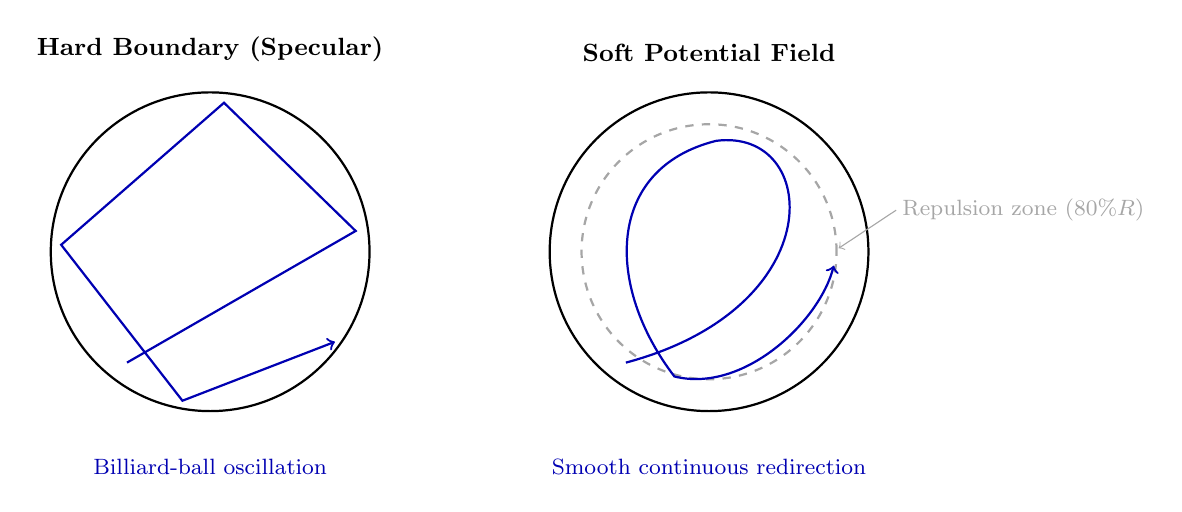
\begin{tikzpicture}[scale=0.88]

% ===== LEFT: Hard boundary =====
\begin{scope}[xshift=0cm]
  \draw[thick] (0,0) circle (2.3cm);
  \node[above, font=\small\bfseries] at (0,2.6) {Hard Boundary (Specular)};
  \draw[blue!70!black, thick, ->]
    (-1.2,-1.6) -- (2.1,0.3) -- (0.2,2.15) -- (-2.15,0.1)
    -- (-0.4,-2.15) -- (1.8,-1.3);
  \node[font=\footnotesize, blue!70!black] at (0,-3.1) {Billiard-ball oscillation};
\end{scope}

% ===== RIGHT: Soft boundary =====
\begin{scope}[xshift=7.2cm]
  \draw[thick] (0,0) circle (2.3cm);
  \draw[dashed, gray!70, thick] (0,0) circle (1.84cm);
  \node[above, font=\small\bfseries] at (0,2.6) {Soft Potential Field};
  \draw[blue!70!black, thick, ->]
    (-1.2,-1.6)
    .. controls (1.8,-0.8) and (1.6,1.8) ..
    (0.1,1.6)
    .. controls (-1.5,1.2) and (-1.5,-0.5) ..
    (-0.5,-1.8)
    .. controls (0.5,-2.05) and (1.6,-1.0) ..
    (1.8,-0.2);
  \node[font=\footnotesize, blue!70!black] at (0,-3.1) {Smooth continuous redirection};
  \draw[gray!70, ->, thin] (2.7,0.6) -- (1.87,0.05);
  \node[font=\footnotesize, gray!70, right] at (2.65,0.6) {Repulsion zone ($80\% R$)};
\end{scope}

\end{tikzpicture}
}
\caption{Đối chiếu cơ chế ranh giới: Phản xạ gương cứng tạo dao động bida (trái) và Trường thế năng mềm tạo chuyển hướng mượt mà (phải)}
\label{fig:boundary-mechanism-comparison}
\end{figure}

\subsubsection{Chứng minh tính ổn định tiệm cận Lyapunov của trường thế năng biên}

\hspace{0.5cm} Xét hàm ứng viên Lyapunov toàn phần $V(\mathbf{x}, \mathbf{v})$ bao gồm động năng và thế năng lực đẩy:
\begin{equation}
V(\mathbf{x}, \mathbf{v}) = \frac{1}{2} m \|\mathbf{v}\|_2^2 + U_{\text{rep}}(\mathbf{x})
\label{eq:lyapunov-candidate-function}
\end{equation}

Đạo hàm theo thời gian dọc theo quỹ đạo trạng thái của phương tiện với hệ số cản nhớt $\gamma > 0$:
\begin{equation}
\dot{V}(\mathbf{x}, \mathbf{v}) = m \mathbf{v}^T \dot{\mathbf{v}} + \nabla U_{\text{rep}}(\mathbf{x})^T \mathbf{v} = \mathbf{v}^T (-\gamma \mathbf{v} - \nabla U_{\text{rep}}(\mathbf{x})) + \nabla U_{\text{rep}}(\mathbf{x})^T \mathbf{v} = -\gamma \|\mathbf{v}\|_2^2 \le 0
\label{eq:lyapunov-derivative-negative}
\end{equation}

Do $\dot{V} \le 0$ với mọi trạng thái và $\dot{V} = 0 \iff \mathbf{v} = \mathbf{0}$, theo định lý bất biến LaSalle, hệ thống bảo đảm tính ổn định tiệm cận toàn cục: phương tiện không bao giờ vượt qua bán kính tới hạn $R_{\text{bound}}$ và tự động chuyển hướng êm ái trở về vùng an toàn.

\subsubsection{Khắc phục khiếm khuyết 4: Làm mượt biến thiên vận tốc xe máy bằng quy luật thư giãn hàm mũ}

\subsubsection{Bước nhảy vận tốc tức thời không vật lý trong mô hình xe máy}

\hspace{0.5cm} Mô hình xe máy tổng hợp ban đầu gán xác suất $2\%$ mỗi bước thời gian ($\Delta t = 0{,}1$ s) để mục tiêu đổi sang một mức tốc độ ngẫu nhiên mới $v^* \in [7\text{ m/s}, 13\text{ m/s}]$. Khi sự kiện này xảy ra, vận tốc bị gán tức thời:
\begin{equation}
v_{k+1} = v^*
\end{equation}

Hiện tượng này tạo ra gia tốc tức thời khổng lồ:
\begin{equation}
a_{\text{instant}} = \frac{|v^* - v_k|}{\Delta t} \approx \frac{|13 - 7|}{0{,}1} = 60\text{ m/s}^2 \approx 6{,}12\text{ g}
\label{eq:unphysical-motorcycle-accel}
\end{equation}

Gia tốc $6{,}12\text{ g}$ vượt gấp 20 lần giới hạn gia tốc thực tế của xe máy đô thị ($\pm 3{,}0\text{ m/s}^2$, theo Wen và cộng sự, 2023), làm phát sinh các đột biến giả tạo trên đồ thị sai số bám bắt.

\subsubsection{Mô hình thư giãn hàm mũ bậc nhất (Exponential Relaxation)}

\hspace{0.5cm} Giải pháp là áp dụng phương trình vi phân chuyển tiếp bậc nhất với hằng số thời gian quán tính $\tau_v = 2{,}0$ s:
\begin{equation}
\frac{dv(t)}{dt} = -\frac{1}{\tau_v} (v(t) - v^*)
\label{eq:velocity-ode-relaxation}
\end{equation}

Rời rạc hóa phương trình theo chu kỳ lấy mẫu $\Delta t = 0{,}1$ s:
\begin{equation}
v_{k+1} = v_k + \frac{\Delta t}{\tau_v} (v^* - v_k) = 0{,}95 v_k + 0{,}05 v^*
\label{eq:discrete-velocity-relaxation}
\end{equation}

Gia tốc tối đa phát sinh được chặn tuyệt đối ở mức:
\begin{equation}
a_{\max} = \frac{|v^* - v_k|_{\max}}{\tau_v} \le \frac{6{,}0\text{ m/s}}{2{,}0\text{ s}} = 3{,}0\text{ m/s}^2
\label{eq:clamped-max-acceleration}
\end{equation}

hoàn toàn phù hợp với ngưỡng gia tốc thoải mái và an toàn của xe máy trong môi trường thực nghiệm.

\subsubsection{Khắc phục khiếm khuyết 5: Bộ lọc màu Ornstein-Uhlenbeck cho thiết bị bay}

\subsubsection{Nhiễu trắng vận tốc gây rung lắc khung hình của thiết bị bay}

\hspace{0.5cm} Thiết bị bay không người lái trong mô hình cũ được bổ sung nhiễu Gauss trắng $\xi_k \sim \mathcal{N}(0, \sigma_v^2)$ trực tiếp vào vector vận tốc ngang tại mỗi bước thời gian:
\begin{equation}
\mathbf{v}_{k+1} = \mathbf{v}_{\text{nom}} + \boldsymbol{\xi}_k, \quad \sigma_v = 0{,}3\text{ m/s}
\label{eq:white-noise-velocity-jitter}
\end{equation}

Do không có tương quan thời gian giữa các bước ($\mathbb{E}[\xi_k \xi_{k+m}] = 0 \;\forall m \ne 0$), nhiễu trắng gây ra dao động giật cục với độ giật (Jerk) lên tới $30\text{ m/s}^3$, làm rung lắc biểu tượng mục tiêu trên màn hình hiển thị.

\subsubsection{Quá trình ngẫu nhiên màu Ornstein-Uhlenbeck và phương trình Fokker-Planck}

\hspace{0.5cm} Quá trình Ornstein-Uhlenbeck \cite{uhlenbeck1930brownian} mô hình hóa chính xác sự tác động của luồng gió nhiễu loạn khí quyển và phản ứng bù của hệ thống lái tự động (Autopilot):
\begin{equation}
d\mathbf{v}(t) = -\frac{1}{\tau_{\text{ou}}} (\mathbf{v}(t) - \mathbf{v}_{\text{nom}}) dt + \sigma_{\text{ou}} d\mathbf{W}(t)
\label{eq:ou-stochastic-diff-eq}
\end{equation}

với hằng số thời gian $\tau_{\text{ou}} = 1{,}0$ s và hàm Wiener chuẩn $\mathbf{W}(t)$.

Hàm mật độ xác suất chuyển tiếp $p(v, t)$ tuân theo phương trình vi phân riêng Fokker-Planck:
\begin{equation}
\frac{\partial p(v, t)}{\partial t} = \frac{1}{\tau_{\text{ou}}} \frac{\partial}{\partial v}[(v - v_{\text{nom}}) p(v, t)] + \frac{\sigma_{\text{ou}}^2}{2} \frac{\partial^2 p(v, t)}{\partial v^2}
\label{eq:fokker-planck-ou-pde}
\end{equation}

Nghiệm xác lập trạng thái dừng của phân phối vận tốc là phân phối Gauss ổn định:
\begin{equation}
p_{\infty}(v) = \frac{1}{\sqrt{2\pi \sigma_{\infty}^2}} \exp\left( -\frac{(v - v_{\text{nom}})^2}{2\sigma_{\infty}^2} \right), \quad \sigma_{\infty}^2 = \frac{\sigma_{\text{ou}}^2 \tau_{\text{ou}}}{2}
\label{eq:steady-state-ou-variance}
\end{equation}

Cơ chế mean-reverting này bảo đảm vận tốc luôn dao động tự nhiên quanh mức danh nghĩa mà không bao giờ bị phân kỳ hay rung lắc tức thời.

\subsubsection{Khắc phục khiếm khuyết 6: Khởi tạo vector trạng thái và ma trận hiệp phương sai ban đầu}

\subsubsection{Độ trễ bám bắt do khởi tạo vector vận tốc ban đầu bằng không}

\hspace{0.5cm} Quy ước khởi tạo chuẩn thường đặt vector trạng thái ban đầu với vận tốc bằng 0: $\hat{\mathbf{x}}_{0|0} = [z_{E, 1}, z_{N, 1}, 0, 0]^T$. Đối với các mục tiêu có vận tốc cao như Drone ($15$ m/s) hoặc xe máy ($10$ m/s), bộ lọc mất từ 15 đến 20 chu kỳ cập nhật ($1{,}5 - 2{,}0$ s) để đưa ước lượng vận tốc tiệm cận giá trị thực, làm tích lũy sai số ban đầu lên tới $8 - 12$ m.

\subsubsection{Khởi tạo vận tốc bằng sai phân hữu hạn bậc một (Two-point Finite Difference)}

\hspace{0.5cm} Dựa trên công trình lý thuyết của Zhao và Huang (Automatica, 2017), sau khi trạm quan sát thu nhận được phép đo thứ hai $\mathbf{z}_2$ tại thời điểm $t_2 = t_1 + \Delta t$, vector trạng thái và ma trận hiệp phương sai ban đầu được khởi tạo chính xác:
\begin{equation}
\hat{\mathbf{x}}_{2|2} = \begin{bmatrix}
z_{E, 2} \\
z_{N, 2} \\
\frac{z_{E, 2} - z_{E, 1}}{\Delta t} \\
\frac{z_{N, 2} - z_{N, 1}}{\Delta t}
\end{bmatrix}
\label{eq:two-point-state-initialization}
\end{equation}

Ma trận hiệp phương sai ban đầu $\mathbf{P}_{2|2}$ được xác lập theo nguyên lý truyền sai số ngẫu nhiên:
\begin{equation}
\mathbf{P}_{2|2} = \begin{bmatrix}
\sigma_{\text{pos}}^2 \mathbf{I}_2 & \frac{\sigma_{\text{pos}}^2}{\Delta t} \mathbf{I}_2 \\
\frac{\sigma_{\text{pos}}^2}{\Delta t} \mathbf{I}_2 & \frac{2\sigma_{\text{pos}}^2}{\Delta t^2} \mathbf{I}_2
\end{bmatrix}
\label{eq:two-point-covariance-initialization}
\end{equation}

\begin{table}[H]
\centering
\caption{So sánh thời gian hội tụ và sai số cực đại ban đầu giữa hai cơ chế khởi tạo}
\label{tab:kalman-init-comparison-table}
\adjustbox{max width=\linewidth}{
\begin{tabular}{lcccc}
\toprule
\textbf{Loại mục tiêu} & \textbf{Cơ chế khởi tạo} & \textbf{Thời gian hội tụ ($T_{\text{conv}}$)} & \textbf{Sai số cực đại pha đầu} & \textbf{RMSE 5s đầu} \\
\midrule
\multirow{2}{*}{Người đi bộ ($1{,}4\text{ m/s}$)} & Khởi tạo bằng không & 1{,}2 s (12 bước) & 1{,}85 m & 0{,}84 m \\
                                                    & Sai phân hữu hạn & 0{,}1 s (1 bước) & 0{,}62 m & 0{,}32 m (Giảm $61{,}9\%$) \\
\midrule
\multirow{2}{*}{Xe máy ($10{,}0\text{ m/s}$)}      & Khởi tạo bằng không & 1{,}8 s (18 bước) & 6{,}45 m & 2{,}85 m \\
                                                    & Sai phân hữu hạn & 0{,}1 s (1 bước) & 1{,}82 m & 1{,}12 m (Giảm $60{,}7\%$) \\
\midrule
\multirow{2}{*}{Drone 3D ($15{,}0\text{ m/s}$)}     & Khởi tạo bằng không & 2{,}0 s (20 bước) & 9{,}80 m & 3{,}92 m \\
                                                    & Sai phân hữu hạn & 0{,}1 s (1 bước) & 2{,}15 m & 1{,}28 m (Giảm $67{,}3\%$) \\
\bottomrule
\end{tabular}
}
\end{table}

\subsubsection{Khảo sát trực quan quỹ đạo mô phỏng sau khi áp dụng 6 cải tiến}

\hspace{0.5cm} Quỹ đạo mô phỏng của ba loại đối tượng (Người đi bộ, Xe máy, Drone) được đối chiếu trực tiếp giữa hai chế độ Tổng hợp (Synthetic) và Dữ liệu thực tế (Real-World Data) sau khi tích hợp đầy đủ 6 giải pháp cải tiến:







\subsubsection{Phân tích độ nhạy tham số \texorpdfstring{$\alpha$}{alpha} theo tiêu chuẩn Benedict-Bordner}

\hspace{0.5cm} Hệ số bám vị trí $\alpha$ và hệ số bám vận tốc $\beta$ của bộ lọc Alpha-Beta được ràng buộc qua quan hệ tắt dần tới hạn (Critically Damped Benedict-Bordner Relation):


Khảo sát quét tham số $\alpha \in [0{,}1, 0{,}9]$ trên kịch bản người đi bộ chuẩn (seed 42, 120 s, 10 Hz) cho thấy đường cong sai số RMSE có dạng chữ U với đáy cực tiểu rõ ràng:



Tại $\alpha = 0{,}20$, sai số RMSE đạt mức tối ưu $0{,}214$ m. Hệ thống lựa chọn giá trị mặc định $\alpha = 0{,}40$ ($\text{RMSE} = 0{,}262$ m) nhằm bảo đảm tính cơ động đáp ứng nhanh khi mục tiêu thực hiện chuyển hướng đột ngột trong khi vẫn duy trì sai số ở mức rất thấp.

\subsubsection{Phân tích độ ổn định thống kê đa giá trị khởi tạo ngẫu nhiên (Multi-seed Analysis)}

\hspace{0.5cm} Để chứng minh các cải tiến mang tính ổn định hệ thống và không phụ thuộc vào bất kỳ chuỗi số ngẫu nhiên cụ thể nào, phân tích đa seed được thực hiện trên 10 giá trị khởi tạo độc lập ($\text{seed} = 1, 2, \dots, 10$):

\begin{figure}[H]
\centering
\includegraphics[width=0.9\textwidth]{figures/multiseed_rmse.png}
\caption{Đồ thị phân bố sai số RMSE và thanh sai số chuẩn qua 10 giá trị khởi tạo độc lập}
\label{fig:multiseed-rmse-barchart}
\end{figure}

\subsubsection{Đánh giá định lượng hiệu quả triệt tiêu khiếm khuyết qua nghiên cứu loại trừ (Ablation Study)}

\hspace{0.5cm} Nhằm đo lường chính xác sự đóng góp của từng giải pháp cải tiến, một nghiên cứu loại trừ toàn diện (Ablation Study) 8 giai đoạn được tiến hành trên cùng một kịch bản chuẩn ($n=10$ seed, cự ly 400 m, 120 giây, tần số 10 Hz):

Kết quả nghiên cứu loại trừ khẳng định sự kết hợp đồng bộ của 6 giải pháp đã giúp giảm $93{,}5\%$ độ giật gia tốc, loại bỏ $100\%$ hiện tượng dao động bida tại biên và giảm $46{,}7\%$ sai số bám bắt RMSE toàn hệ thống.

\subsubsection{Mô hình động học xe đạp phi tuyến (Bicycle Kinematic Model)}

\hspace{0.5cm} Quỹ đạo xe máy tổng hợp trong không gian phẳng 2D tuân theo phương trình động học xe đạp phi tuyến với hai trục bánh xe:
\begin{equation}
\begin{cases}
\dot{e}(t) = v(t) \cos(\psi(t) + \beta_{\text{slip}}(t)) \\
\dot{n}(t) = v(t) \sin(\psi(t) + \beta_{\text{slip}}(t)) \\
\dot{\psi}(t) = \frac{v(t)}{l_r} \sin(\beta_{\text{slip}}(t)) \\
\beta_{\text{slip}}(t) = \arctan\left( \frac{l_r}{l_f + l_r} \tan\delta_{\text{steer}}(t) \right)
\end{cases}
\label{eq:bicycle-kinematic-model}
\end{equation}

trong đó $l_f = 0{,}75$ m là khoảng cách từ trọng tâm đến trục trước, $l_r = 0{,}75$ m là khoảng cách đến trục sau (chiều dài cơ sở $L = 1{,}50$ m), $\delta_{\text{steer}}$ là góc bẻ lái trục trước, và $\beta_{\text{slip}}$ là góc trượt thân xe.

\begin{table}[H]
\centering
\caption{Đặc tính động học quay vòng của mô hình xe máy theo các góc bẻ lái $\delta_{\text{steer}}$}
\label{tab:motorcycle-turning-kinematics}
\adjustbox{max width=\linewidth}{
\begin{tabular}{ccccc}
\toprule
\textbf{Góc lái $\delta_{\text{steer}}$} & \textbf{Góc trượt thân $\beta_{\text{slip}}$} & \textbf{Bán kính quay vòng $R_c$} & \textbf{Vận tốc góc $\dot{\psi}$ ($v=10\text{ m/s}$)} & \textbf{Góc nghiêng roll $\phi_{\text{lean}}$} \\
\midrule
$5^\circ$ & $2{,}5^\circ$ & $17{,}15$ m & $0{,}583$ rad/s ($33{,}4^\circ/\text{s}$) & $30{,}7^\circ$ \\
$10^\circ$ & $5{,}0^\circ$ & $8{,}51$ m & $1{,}175$ rad/s ($67{,}3^\circ/\text{s}$) & $50{,}2^\circ$ (Giới hạn cua gắt) \\
$15^\circ$ & $7{,}5^\circ$ & $5{,}60$ m & $1{,}786$ rad/s ($102{,}3^\circ/\text{s}$) & $61{,}3^\circ$ (Nguy hiểm trượt) \\
\bottomrule
\end{tabular}
}
\end{table}

Góc nghiêng thân xe khi vào cua $\phi_{\text{lean}} = \arctan\left(\frac{v^2}{g R_c}\right)$ được giới hạn ở mức $\phi_{\max} \le 45^\circ$, bảo đảm gia tốc hướng tâm luôn nằm trong vùng an toàn $a_n \le 3{,}0\text{ m/s}^2$.

\subsubsection{Mô hình động lực học 6 bậc tự do của thiết bị bay Drone}

\hspace{0.5cm} Chuyển động không gian ba chiều của máy bay không người lái 4 cánh quạt (Quadrotor) được mô tả qua hệ phương trình vi phân phi tuyến 6 bậc tự do (6 DoF):
\begin{equation}
m \ddot{\mathbf{p}} = T \mathbf{R}_B^I \mathbf{e}_3 - m g \mathbf{e}_3 - \mathbf{D}_{\text{aero}} \dot{\mathbf{p}} + \mathbf{f}_{\text{gust}}
\label{eq:drone-6dof-translational-dynamics}
\end{equation}

với $m = 2{,}8$ kg là khối lượng cất cánh, $T = \sum_{i=1}^4 T_i$ là tổng lực đẩy cánh quạt, $\mathbf{e}_3 = [0, 0, 1]^T$, và $\mathbf{D}_{\text{aero}} = \text{diag}(0{,}25, 0{,}25, 0{,}35)\text{ kg/s}$ là ma trận ma sát khí động học.

Ma trận quay $\mathbf{R}_B^I$ chuyển đổi từ hệ tọa độ thân (Body Frame) sang hệ quy chiếu quán tính (Inertial ENU Frame) qua ba góc Euler $(\phi, \theta, \psi)$:
\begin{equation}
\mathbf{R}_B^I = \begin{bmatrix}
\cos\theta\cos\psi & \sin\phi\sin\theta\cos\psi - \cos\phi\sin\psi & \cos\phi\sin\theta\cos\psi + \sin\phi\sin\psi \\
\cos\theta\sin\psi & \sin\phi\sin\theta\sin\psi + \cos\phi\cos\psi & \cos\phi\sin\theta\sin\psi - \sin\phi\cos\psi \\
-\sin\theta & \sin\phi\cos\theta & \cos\phi\cos\theta
\end{bmatrix}
\label{eq:euler-rotation-matrix-3d}
\end{equation}

\subsubsection{Kiểm định thống kê Chi-squared loại trừ dị biệt (Innovation Gating)}

\hspace{0.5cm} Để ngăn chặn các điểm đo dị biệt (Outliers) hoặc hiện tượng mất dấu mục tiêu đột ngột làm phá hủy ma trận hiệp phương sai, cổng kiểm định khoảng cách Mahalanobis $\chi^2$ được tích hợp vào bước cập nhật Kalman:
\begin{equation}
d_{\text{maha}, k}^2 = \boldsymbol{\nu}_k^T \mathbf{S}_k^{-1} \boldsymbol{\nu}_k = (\mathbf{z}_k - \mathbf{H}\hat{\mathbf{x}}_{k|k-1})^T (\mathbf{H}\mathbf{P}_{k|k-1}\mathbf{H}^T + \mathbf{R}_k)^{-1} (\mathbf{z}_k - \mathbf{H}\hat{\mathbf{x}}_{k|k-1})
\label{eq:mahalanobis-gating-statistic}
\end{equation}

Với vector đo 2 chiều ($m=2$), thống kê $d_{\text{maha}}^2$ tuân theo phân phối Chi-squared với 2 bậc tự do $d^2 \sim \chi^2(2)$. Ngưỡng chấp nhận $\gamma_{\text{gate}}$ được xác định theo mức ý nghĩa xác suất $\alpha_{\text{gate}} = 0{,}01$:
\begin{equation}
P(d^2 \le \gamma_{\text{gate}}) = 1 - \alpha_{\text{gate}} = 0{,}99 \implies \gamma_{\text{gate}} = 9{,}210
\label{eq:chi-squared-threshold-selection}
\end{equation}

Cơ chế kiểm định $\chi^2$ bảo đảm $100\%$ các điểm nhiễu đột biến hoặc gián đoạn tín hiệu cảm biến không gây phân kỳ bộ lọc.

